\subsection{Verification and Validation on Classical B model}

The first section \ref{sec:processes} describes usual verification and validation activities applied during the design of industrial critical software using the B method. Second section \ref{sec:tools} gives a description of tools available.

Last section \ref{app:osproc} describes the results on an example.


\subsubsection{Verification processes applicable to a B~model}
\label{sec:processes}

A B~model is a textual and formal specification covering the functional behaviour of a safety critical software. It is usually written based on a high-level specification (informal or formal specification, for example SysML or a natural language). It is gradually refined, starting at the top with an abstract notation and ending at the bottom with sequential instructions --- which are then automatically translated in a target language such as C or Ada.\\
Thus, we define three objects of verification and validation: the specification, the B~model and the generated source code.\\


Validation consists of:
\begin{itemize}
\item guaranteeing the functional adequacy between the specification and the model (this can be achieved, for example, through review and proofreading),
\item building a test environment around the generated source code and test it.
\end{itemize}
Hence, this section will mainly focus on verification, i.e.\ the methods and tools required to assure that B~method is a consistent way of producing critical software.

In this section, we demonstrate the suitability of the B~method towards the problematics encountered in the openETCS project by introducing the different verification processes applicable to a B~model.\\
Each of the verification process is presented and its contributions to the system security and consistency are discussed.

\paragraph{Type checking}
Static type checking (TC) is a basic form of program verification that ensures type safety of the model. It is the first verification --- after lexical and syntactic analysis --- to be performed on a B~model, thus allowing an early detection of problems. It is also a pre-requisite for the higher-level verifications. \\
Strong typing ensures a consistent use of data and is essential to writing correct formulae (predicates or expressions).\\

The type checking process consists of two main activities: data typing and type verification.\\
{\itshape Data typing} is the activity of assigning a type to newly-encountered data in a predicate or a substitution. {In B, a substitution is comparable to a set of instructions that modify variables. For more information, see \cite{bbook}}. It is based on an inference mechanism, which is able to deduce the type of a newly-encountered variable from the type of the other variables intervening in the predicate or the substitution, and specific inference rules.\\
On the other hand, {\itshape type verification} is the activity of verifying typing rules between already-typed variables. These rules are specific to their applying predicates, expressions or substitutions.
% In B, the base types consist of integers, booleans, strings, abstract sets and enumerated sets.\\
% The construction of more complex types is achieved through the powerset operator $\mathbb{P}$ and the cartesian product $\times$.

\paragraph{B0-check}
The B0 verification has the specific purpose of checking the respect of the rules that the B~model has to conform to in order to generate the translation to C or ADA. These rules are called implementability rules and must be respected in order for the translation to process properly. They also ensure that the resulting code is executable and respects a set of properties.

\paragraph{Well-definedness}
An expression is well-defined (WD) if its associated value or interpretation exists and is unique, thus avoiding ambiguity.\\
Examples of ill-defined formulae include division by zero, function application to an argument out of the domain, function application of a relation etc.\\

Well-definedness checking is thus an extra verification that helps strengthen the model.

\paragraph{Model checking}

Model checking is a static semantic check that searches for invariant or
assertion violations and deadlock states. It exhaustively explores the whole
state space, i.e., is in general limited to finite systems.\\
This type of verification animates the model, modifying the current state of the
machine, starting from the initialization. Operation calls are simulated and
modify the internal state which is then checked for various properties. Most of
the time, an invariant or assertion violation is looked for.\\
This verification process, as opposed to the ones previously introduced,
considers the semantics of the model and aims at verifying properties
dynamically. However, it has its limitations:
\begin{itemize}
\item inability to run through all of the states and transitions for models with
  infinitely many states
\item difficulty to deal with very large models or large domains (e.g. 32~bit
  integers) often leading to state-space explosion because of exponential growth
  of the state space size.
\end{itemize}
This means that potential erroneous states can be missed, and that this
verification process is not sufficient to ensure \textit{correctness}, though
satisfying as an additional verification tool.

\paragraph{Constraint-based checking}

Constraint-based checking (CBC) is the process of finding a given valid state, for which an operation call leads to an erroneous state. This is done by constraint solving instead of --- as seen for model checking --- running through states from the initialization.\\
This technique will usually provide more counter-examples than model-checking, because it ignores the initialization constraints and can thus reach a wider range of states.

\paragraph{Formal proof}
A proof obligation is a mathematical lemma generated by the proof obligation
generator (POG). It corresponds to a consistency property of the model, that has
to be demonstrated. These properties are either generated to ensure correctness
of the model, e.g., refinement, variable typing, well-definedness or they are
specified manually as invariants of the system, e.g., dependent typing, safety
invariants. A fully-proved model is said to be \textit{correct}, in the sense
that every property (invariant, assertion) expressed is proved to hold for every
state of the program. If a proof obligation is not provable, it means that the
B~model is inconsistent and must be corrected. In fact, the goal of any B
development is to obtain a proved model.\\
In contrast to model-checking, formal proof does not require to make assumptions
about the size of the system (number of transitions). It is reliable and
powerful, but it needs to be taken into account that:
\begin{itemize}
\item some proofs can be very difficult to solve,
\item the model needs to be written as to make it the simplest to prove, which demands experience and skill.
\end{itemize}
A proved model will always meet the formalized safety and security
qualifications~; however that does not mean it will behave in regards to the
informal specification! It must be validated that the formalized specification
(and in consequence the formalized model) correctly implements the informal
specification, in particular that the intended functioning is possible. This is
the domain of validation, as discussed in the introduction.

\subsubsection{Tools}
\label{sec:tools}

%\subsubsection{Existing tools}
In this section, we present the existing tools suitable for the verification processes defined in Section~\ref{sec:processes}.

\paragraph{Atelier~B}
\label{subsec:atelierb}
Atelier B\footnote{See \url{http://www.atelierb.eu/en}} is the main development tool associated with the B~method and is produced and distributed by ClearSy. It provides most of the needed tools.

\paragraph{B~compiler}~\\
The B~compiler performs syntax analysis, type checking, identifier scope resolution and B0-checking. It is part of Atelier~B as an open source tool.

\paragraph{Proof obligation generator}~\\
Atelier~B's POG is currently the only known fully operational POG for B, and is free of charge --- although proprietary software, which means closed-source. ClearSy is currently working on a new proof obligation generator~; whether it will be open source or not is to be determined.

\paragraph{Prover, proof assistant, user-defined rules}~\\
Atelier~B provides a free of charge --- although not open source --- prover which discharges proof obligations. Depending on the complexity of the model, a varying proportion of the proof obligations is discharged automatically.\\
For the remaining proof obligations, Atelier~B provides an interactive proof assistant allowing the user to guide the prover in discharging the PO. The user may define theories (or rules) which have in turn to be proved. The user-defined rules are organized in a database and can be automatically verified and validated with the Rule Verifier of Atelier~B.

\paragraph{Atelier~B translators}~\\
Translators are an essential component of the industrial success of B. The translators take the B0 implementations as input and produce a target source code, typically Ada or C/C++, ready to be compiled or integrated in an environment.\\
ClearSy provides an open source translator, but it does not reach the T3 level of qualification\footnote{For additional information on qualification, see subsection \ref{subsec:qualif} or the CENELEC norm.}.

\paragraph{ProB}
\label{subsec:prob}
ProB is an animator and model checker for B~models distributed under the EPL license (open source) and mainly developed by Formal Mind\footnote{See \url{http://www.formalmind.com}}.\\
It performs model checking as well as constraint-based checking and searches for a range of errors, with customizable search options and various graphical views. ProB also handles automatic coverage reports generation.\\
ProB is a mature tool and is being used by several industrials such as Siemens and Alstom. This makes it a precious tool for the verification processes described above.

\paragraph{Tool qualification}
\label{subsec:qualif}
Atelier~B has been used for many years to develop railway critical software. It is, for this exact reason, {\itshape qualified} by the main actors of the railway domain: SNCF, RATP, Alstom, Siemens etc.\\

The CENELEC norm defines qualification levels for verification tools. Annex A 5 of the norm specifies several verification techniques and for each of them, a recommendation level (mandatory, highly recommended, recommended). Below are listed the different techniques and measures along with their recommendation levels for SIL4 developments~: Recommended, Highly Recommended or Mandatory.

Table \ref{tab:cenelec} shows, for each of the verification processes presented in \ref{sec:processes} (specification and source code were added as artifacts which support the activity), the corresponding item in the CENELEC norm annex table.

\begin{table}[h!]
\begin{center}
\scalebox{.88}{
\begin{tabular}{@{}l l l c c c c c c c@{}}
~ & ~ & level & spec & TC & B0C & MC & CBC & proof & source code \\
\hline
A 5.1 & Formal Proof & HR & ~ & ~ & ~ & ~ & ~ & \checkmark & ~ \\
\hline
A 5.2 & Static Analysis & HR & ~ & \checkmark & \checkmark & ~ & \checkmark & ~ & ~ \\
\hline
A 5.3 & Dynamic Analysis and Testing & HR & ~ & ~ & ~ & \checkmark & ~ & ~ & ~ \\
\hline
A 5.4 & Metrics & R & ~ & ~ & ~ & ~ & ~ & ~ & ~ \\
\hline
A 5.5 & Traceability & M & \checkmark & ~ & ~ & ~ & ~ & \checkmark & ~ \\
\hline
A 5.6 &  Software Error Effect Analysis & HR & ~ & ~ & ~ & ~ & ~ & ~ & ~ \\
\hline
A 5.7 & Test Coverage for code& HR & ~ & ~ & ~ & ~ & ~ & ~ & ~ \\
\hline
A 5.8 & Functional/ Black-box Testing & M & ~ & ~ & ~ & ~ & ~ & ~ & \checkmark \\
\hline
A 5.9 & Performance testing & HR & ~ & ~ & ~ & ~ & ~ & ~ & ~ \\
\hline
A 5.10 & Interface testing & HR & ~ & ~ & ~ & ~ & ~ & ~ & ~ \\
\hline
\end{tabular}}
\end{center}
\caption{Correspondence between CENELEC norm recommendations and the presented verification processes}
\label{tab:cenelec}
\end{table}

A B~model proof provides a formal proof in the form of a proof tree that can be
inspected by humans and is machine-checkable, i.e., an automated program can
replay the proof steps and verify the correct application of the proof rules.\\
Static type checking, B0 compliance for programming language translation and
constraint based checking do not require any dynamic, i.e., state-space
information to detect problems. Therefore these representing static analysis
approaches of B~model.\\
Model checking analyzes the dynamic behavior of the model by generating and
exploring the state-space. Very often, model checkers can generate
counter-examples for violated properties and can therefore be applied as a
testing method.\\
The specification in the B~model represents a formalized version of the
specification, the proof trees use formalized properties as proof steps. These
can be traced in the informal specification.\\
Finally the translated source code can be compiled and tested using various
testing methods, including functional tests and black-box testing.

\paragraph{Conclusion on tools}
Table \ref{tab:comparison} summarizes the presentation of the tools in subsections \ref{subsec:atelierb} and \ref{subsec:prob}.\\
Atelier~B and ProB are both mature tools that have proved their worth. They are the core tools for validation processes of B~models. However, key components of Atelier~B are not open source and this issue is not completely compensated by ProB's model checking and CBC.\\
An ongoing research project named BWare\footnote{See \url{http://bware.lri.fr/index.php/BWare_project}} and conducted by ClearSy, Inria, LRI and others aims at providing a framework from proof obligation generation to proof discharge by the means of SMT solvers. This promising project started in September 2012 and is funded for a period of four years. It opens perspectives for the near future in terms of open source B~model verification.

\begin{table}[h!]
\begin{center}
\begin{tabular}{l c c c c c}
~ & TC & B0 & model check. & CBC & proof \\
\hline
B~Compiler & \checkmark & \checkmark & ~ & ~ & ~ \\
\hline
POG and provers & ~ & ~ & ~ & ~ & \checkmark \\ 
\hline
ProB & ~ & ~ & \checkmark & \checkmark & ~ \\
\hline
\end{tabular}
\end{center}
\caption{Comparison of the tools available for B verification processes}
\label{tab:comparison}
\end{table}

%\appendix
\subsubsection{Application: Procedure On-Sight}
\label{app:osproc}
The Procedure On-Sight, as described in {\itshape System Requirements Specification, Chapter 5}, has been modelled in B\footnote{The model is available at \url{github.com/openETCS/validation/tree/master/VnVUserStories/VnVUserStorySysterel/02-DAS2V/c-ClassicalBModel/ProcedureOnSight}.} to show the feasibility of the task and the credibility of the method. This appendix briefly presents the model, then applies the verification processes to this example.

\paragraph{Presentation of the B~model}
As shown in figure \ref{fig:procos}, the model is split into three main processing modules, one of which corresponds to the actual on-sight procedure,
and the two others being used as data conditioning:
\begin{itemize}
\item \verb+os_mode_level+: determines the ETCS level and the mode. Contains the on-sight procedure algorithm,
\item \verb+os_consist+: checks data consistency, provides adaptation to the current ETCS level (BTM or radio),
\item \verb+os_train_info+: elaborates the location and the speed of the train.
\end{itemize}

\begin{figure}[h!]
\centering
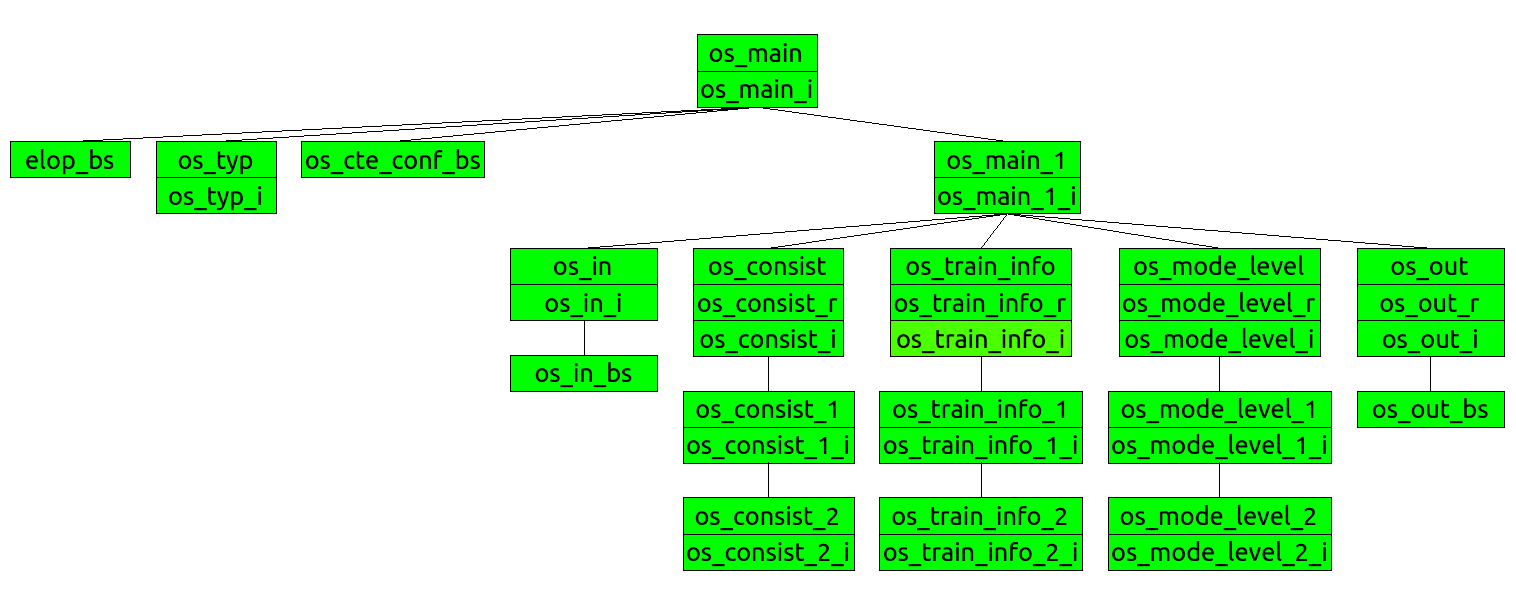
\includegraphics[width=1\textwidth]{figures/procedureos}
\caption{Architecture of the B~model for the Procedure On-Sight example}
\label{fig:procos}
\end{figure}

These three modules are imported by the main sequencer, \verb+os_main_1+, which calls their respective operations. The main sequencer also imports the input module \verb+os_in+, and the output module \verb+os_out+.\\
The typing machine, \verb+os_typ+, and the constant machine, \verb+os_cte_conf_bs+, are both imported by \verb+os_main+, the entry point of the software, which also imports \verb+os_main_1+.\\
 
This ``IMPORTS''-based vertical layout is complemented by a horizontal aspect: the ``SEES'' clause, which enables a component to access another component's data. It is possible for a component to see the components to its left, but not to its right. Thus, a cycle-free graph is maintained.
 
\paragraph{Model checking results}
\label{subapp:mc}
ProB has been used on the example model and has shown through model checking that no invariant was violated, and no deadlock state was found. However, for some machines, only a minority of states and nodes have been visited (because of infinite sets in particular) and thus no formal conclusion can be drawn.\\
Additionally, constraint-based checking has also been run and stated, for every operation of every abstract machine, the non-violation of the invariant.

\paragraph{Formal proof results}
\label{subapp:proof}

%\subparagraph{Project status}
Project status illustrated in figure \ref{fig:atelierb} shows the fully-proved model in Atelier~B. 

\begin{figure}[h!]
\centering
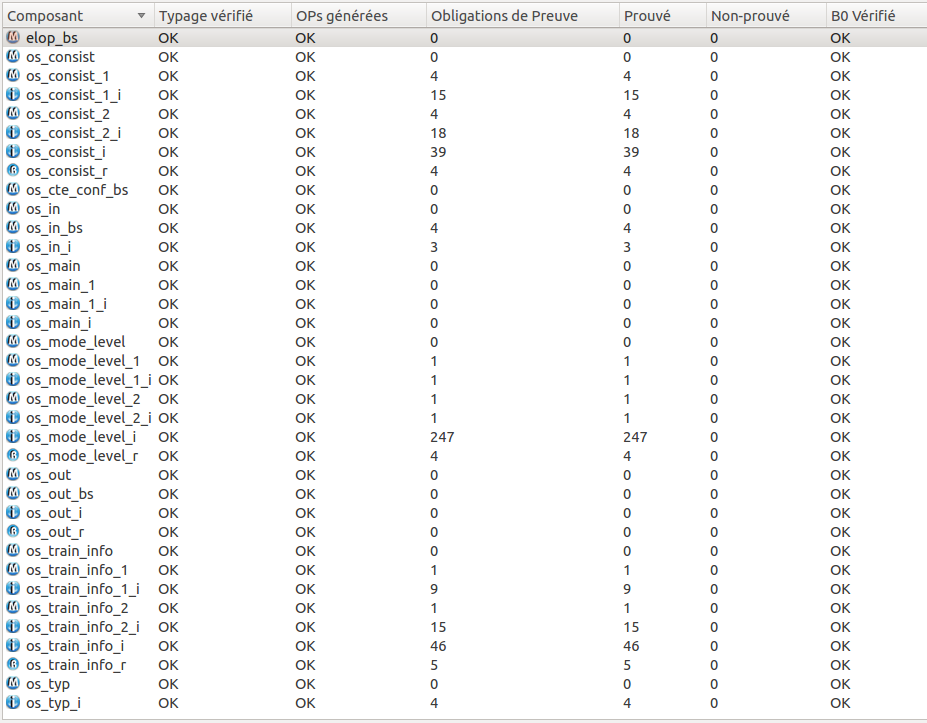
\includegraphics[width=1\textwidth]{figures/atelierb}
\caption{Overview of the B~model in Atelier~B, showing type check, B0 check and proof status}
\label{fig:atelierb}
\end{figure}

This model was proved almost entirely automatically, using the provers with
force 0 and force 1 (on 427 proof obligation generated, only 3 need the
interactive prover to define cases). Proving the model results in the certainty
of its correctness wrt.\ the formal specification. In this case, only typing
invariants and constraints were expressed, because more complex safety
properties have not been identified to be specified as invariant. However, for each function, its behaviour is specified and the implementation is verified according to this specification.

%\subparagraph{User-defined theories}
When automatic proof fails, the user must provide a manual proof and uses theories for this purpose. Theories are rules that are used to discharge specific goals.\\
In this example, the only module for which interactive proof was required is \verb+os_consist_i+. Below is presented a very simple theory (among several others) used for the proof of this component:

\begin{equation}
\tag{User theory 1}
a < 0 \land 0 \leq b \land 0 < c \Rightarrow a \leq \frac{b}{c}
\end{equation}

This theory is automatically verified by Atelier~B and therefore ensures full consistency of the proof.


\subsubsection{Conclusion}
The B~method, along with its verification processes and tools, meets the goals and activities of the openETCS project in terms of quality, rigor, safety and credibility.\\
There is yet to develop open-source POG and build a framework for proving, but this is compensated by the fact that work on the subject is ongoing, and ProB is an effective tool for verification.

